\part{Lecture 14: Outlook and Research Insights}
\title[RL Lecture 14]{Lecture 14: Outlook and Research Insights}
\date{}  
\frame{\titlepage} 

%%%%%%%%%%%%%%%%%%%%%%%%%%%%%%%%%%%%%%%%%%%%%%%%%%%%%%%%%%%%%%%%%%
\section{Safe Reinforcement Learning} 
%%%%%%%%%%%%%%%%%%%%%%%%%%%%%%%%%%%%%%%%%%%%%%%%%%%%%%%%%%%%%%%%%%
\begin{frame}
\frametitle{Table of contents}
\tableofcontents[currentsection]
\end{frame}

%%%%%%%%%%%%%%%%%%%%%%%%%%%%%%%%%%%%%%%%%%%%%%%%%%%%%%%%%%%%%
%% Recap: optimal control and constraints %%
%%%%%%%%%%%%%%%%%%%%%%%%%%%%%%%%%%%%%%%%%%%%%%%%%%%%%%%%%%%%%
\frame{\frametitle{Recap: optimal control and constraints}
Real-world systems are always subject to certain state constraints $\mathcal{X}$ and input limitations $\mathcal{U}$. Violating those can lead to safety issues.   
\begin{equation}
	\begin{split}
	v_k^* &= \max_{\bm{u}_k} \sum_{i=0}^{N_\mathrm{p}} \gamma^i r_{k+i+1} (\bm{x}_{k+i}, \bm{u}_{k+i})\, ,\\
	\mathrm{s.t.} \quad\quad \bm{x}_{k+i+1}&=\bm{f}(\bm{x}_{k+i},\bm{u}_{k+i}), \quad \bm{x}_{k+i} \in \mathcal{X},\quad \bm{u}_{k+i} \in \mathcal{U}\,.\\
\end{split}
\end{equation}
\begin{figure}
\centering
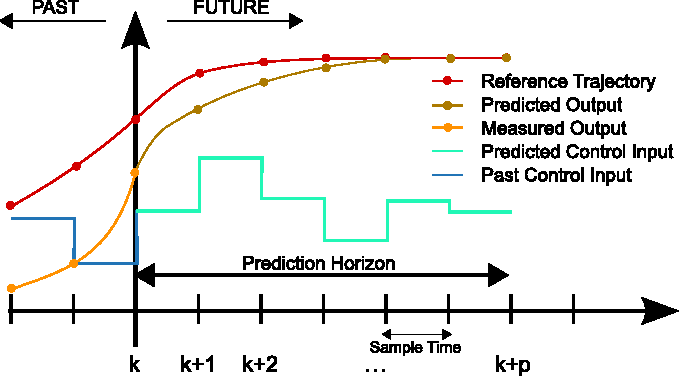
\includegraphics[height=0.4\textheight]{fig/lec01/MPC.pdf}
\caption{MPC scheme (source: \href{https://de.wikipedia.org/wiki/Model_Predictive_Control}{www.wikipedia.org},  by Martin Behrendt \href{https://creativecommons.org/licenses/by-sa/3.0/deed.en}{CC BY-SA 3.0})}
\label{fig:MPC}
\end{figure}
}

%%%%%%%%%%%%%%%%%%%%%%%%%%%%%%%%%%%%%%%%%%%%%%%%%%%%%%%%%%%%%
%% Application examples with safety concerns %%
%%%%%%%%%%%%%%%%%%%%%%%%%%%%%%%%%%%%%%%%%%%%%%%%%%%%%%%%%%%%%
\frame{\frametitle{Application examples with safety-relevant constraints}
\begin{figure}
 \centering
 \begin{columns}
        \column{.2\linewidth}
				\caption*{Collaborative robot control (source: \href{https://commons.wikimedia.org/wiki/File:Human-Robot-Collaboration-Sawing-2016-Luka-Peternel.jpg}{www.wikipedia.org}, \href{https://creativecommons.org/licenses/by-sa/4.0/deed.en}{CC BY-SA 4.0})}
        \column{.3\linewidth}
        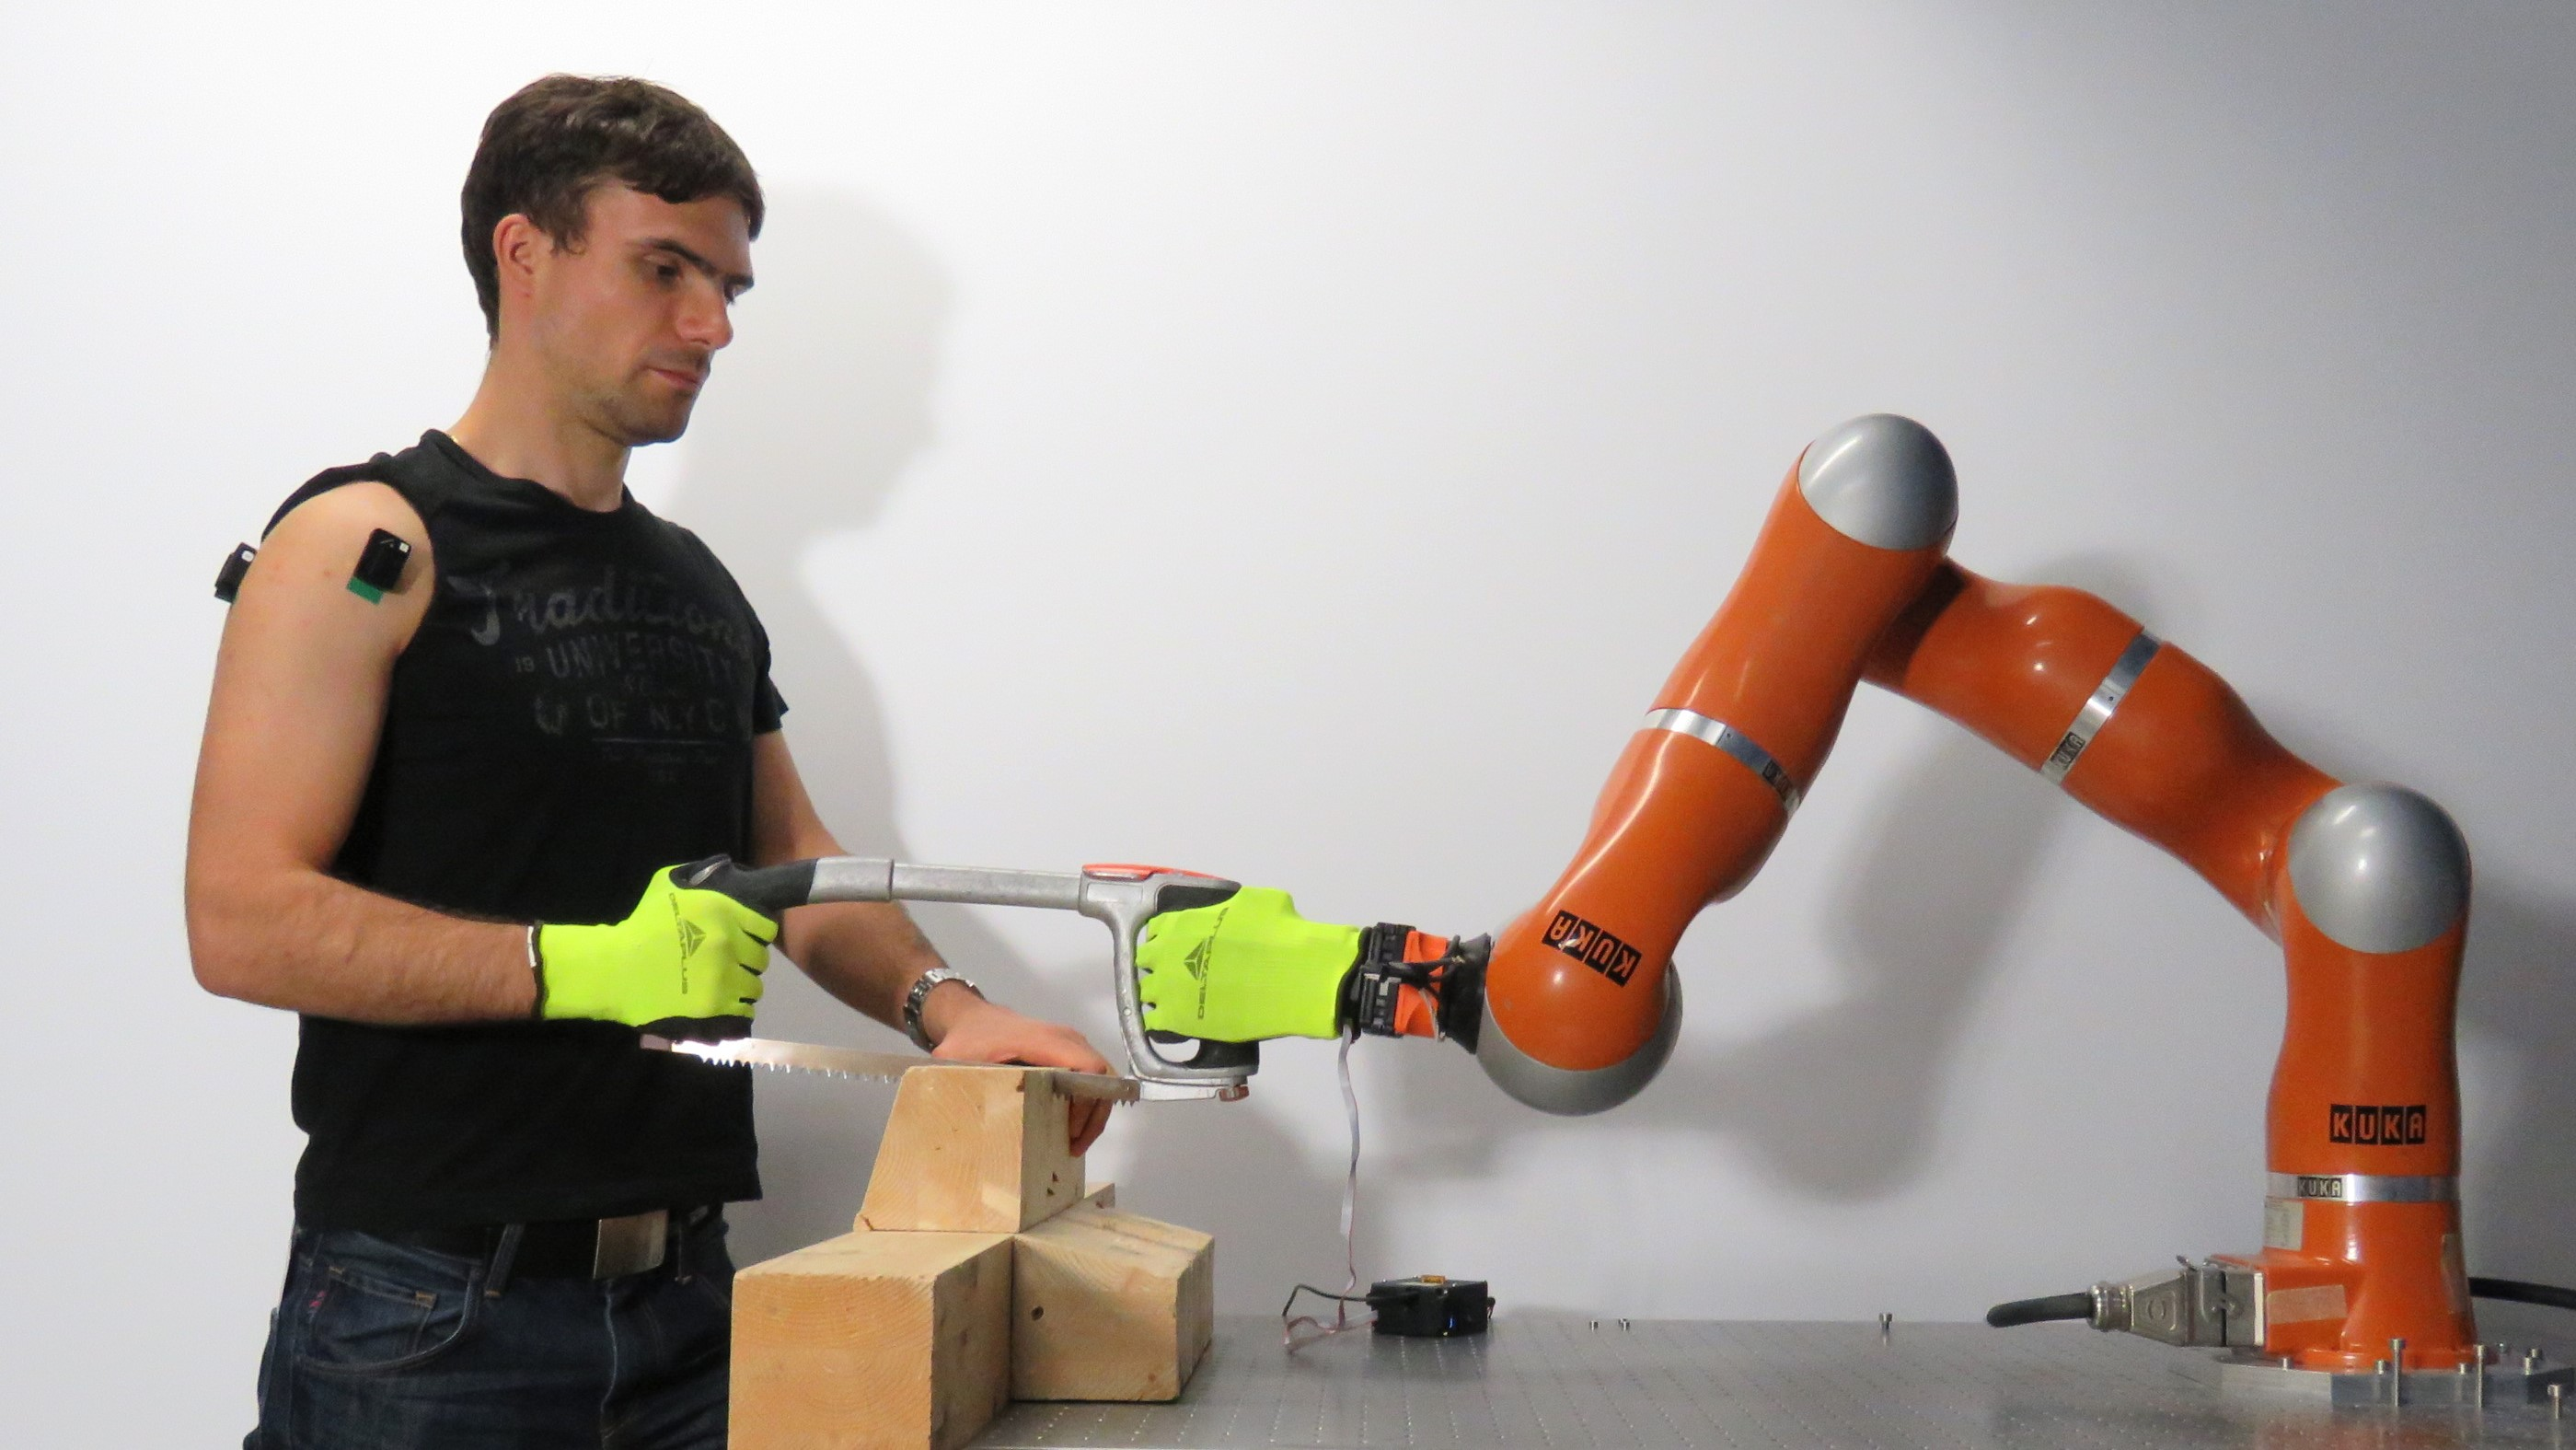
\includegraphics[width=\textwidth]{fig/lec14/Human-Robot-Collaboration.jpg}
				\column{.3\linewidth}
        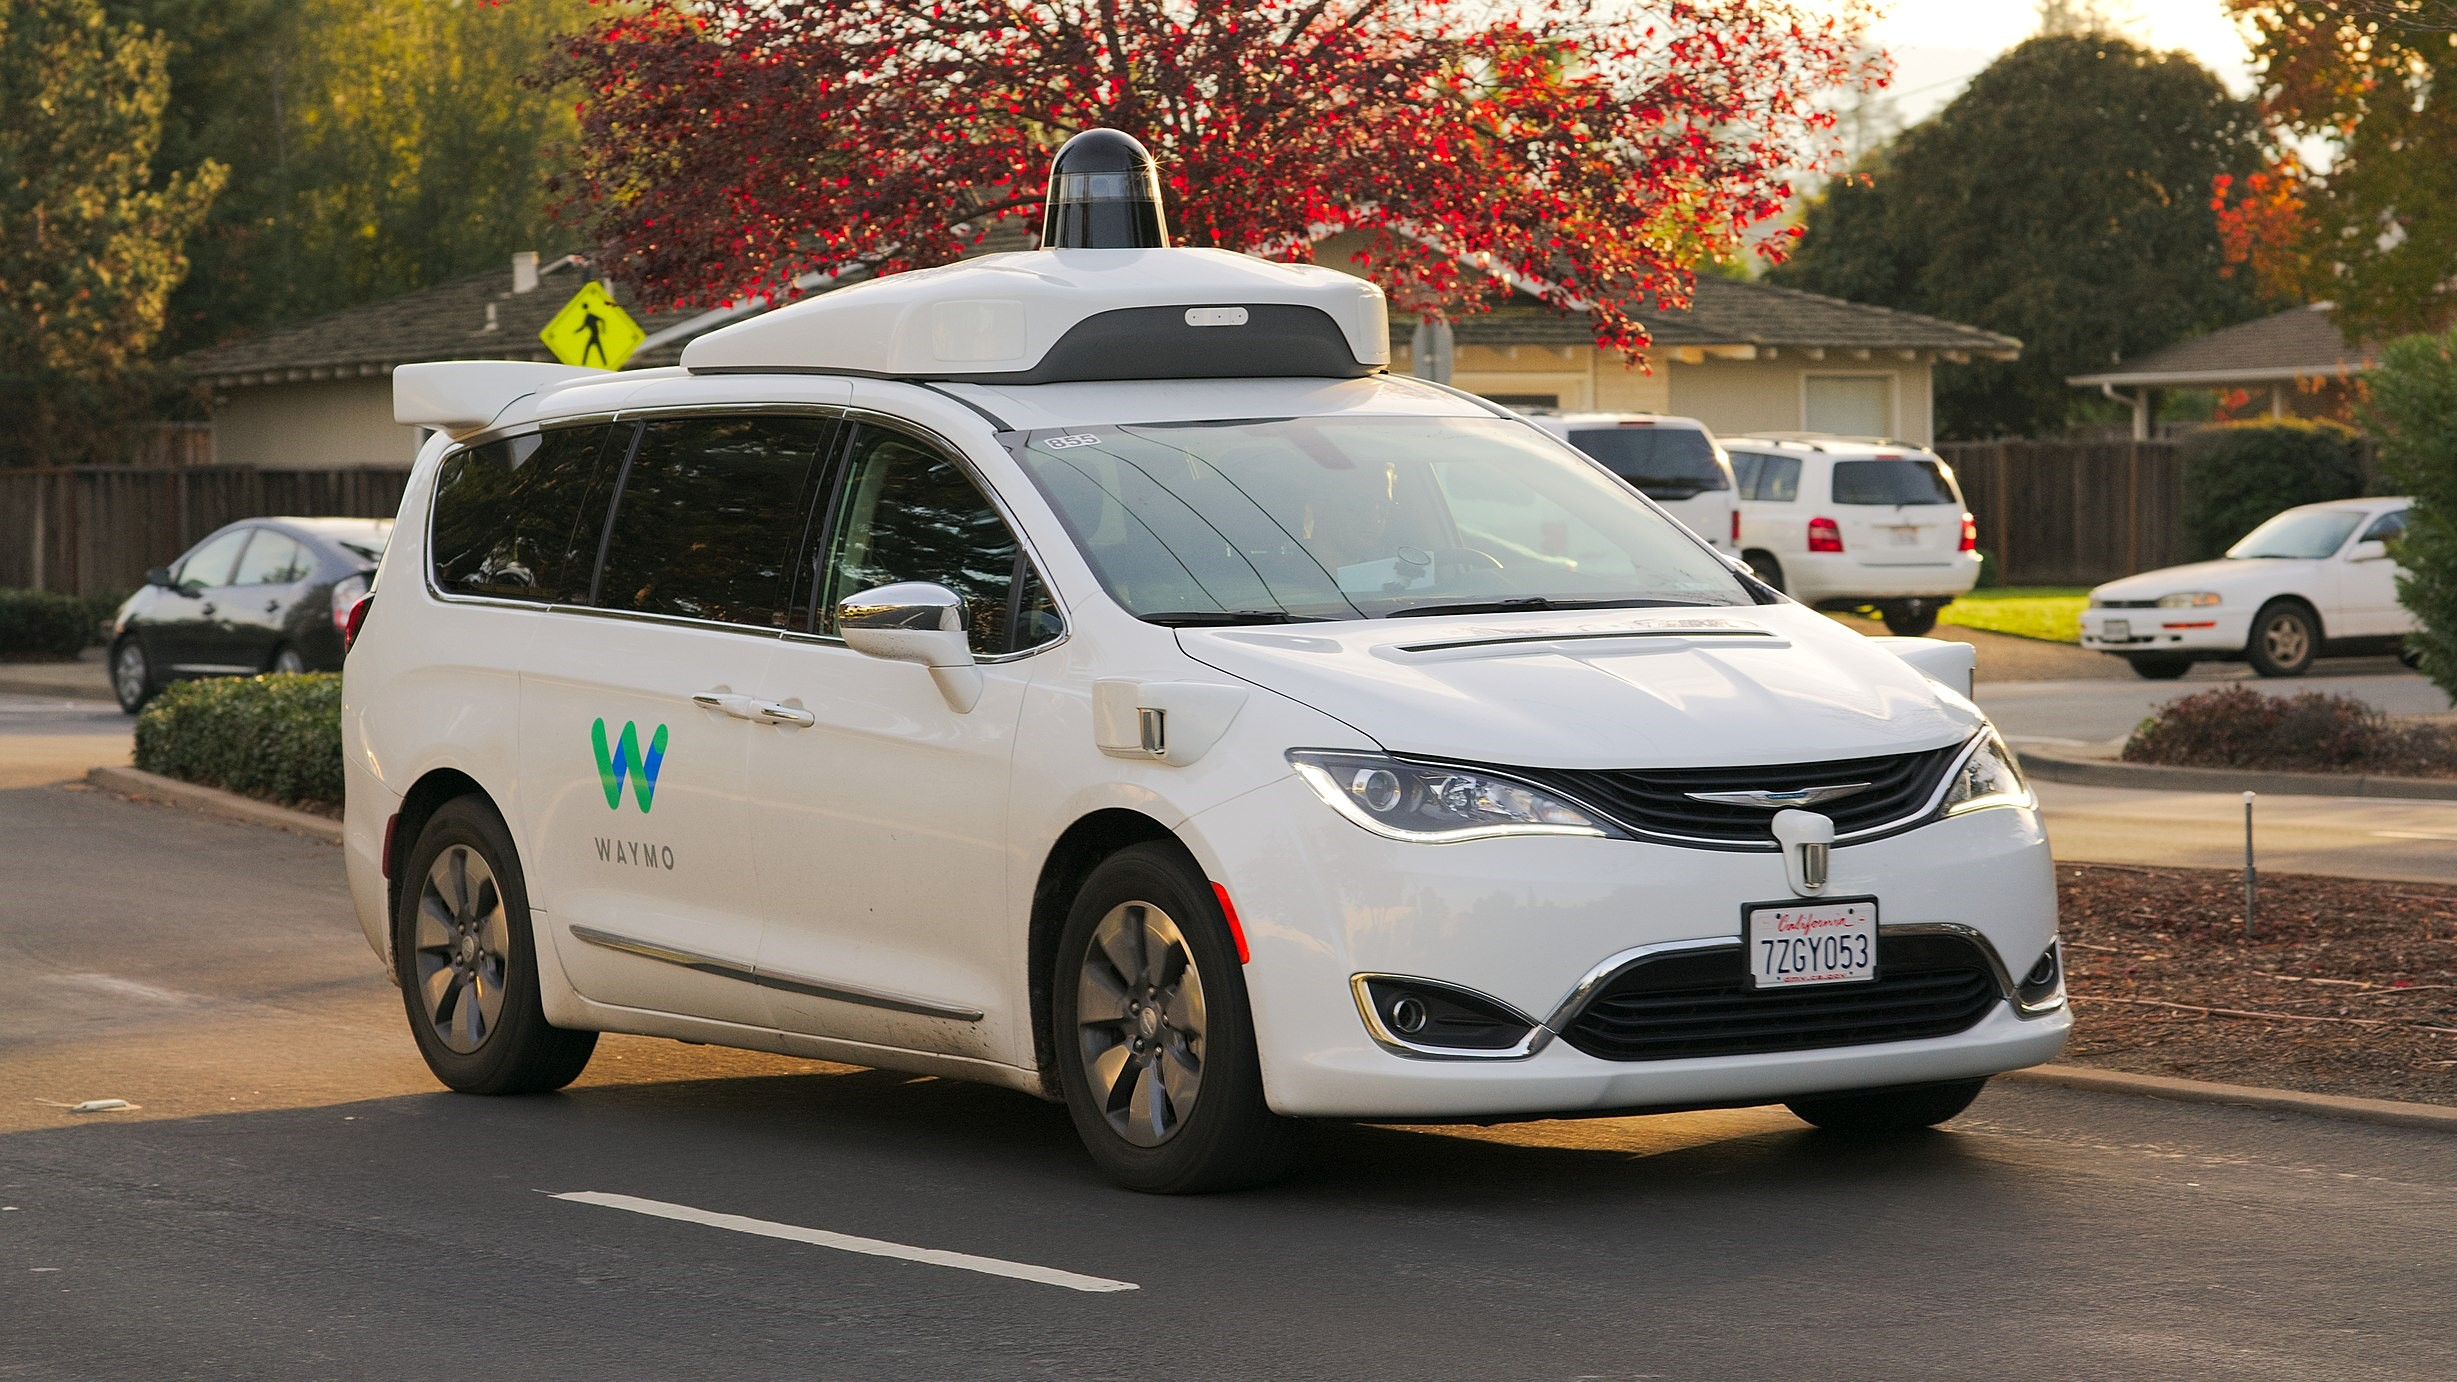
\includegraphics[width=\textwidth]{fig/lec14/Waymo.jpg}
				\column{.2\linewidth}
				\caption*{Autonomous car driving (source: \href{https://commons.wikimedia.org/wiki/File:Waymo_Chrysler_Pacifica_in_Los_Altos,_2017.jpg}{www.wikipedia.org}, \href{https://creativecommons.org/licenses/by-sa/4.0/deed.en}{CC BY-SA 4.0})}
      \end{columns}
			\vspace{1cm}
			\begin{columns}
        \column{.2\linewidth}
				\caption*{Energy system control}
        \column{.3\linewidth}
        \includegraphics[width=\textwidth]{fig/lec14/microgrid.jpg}
				\column{.3\linewidth}
        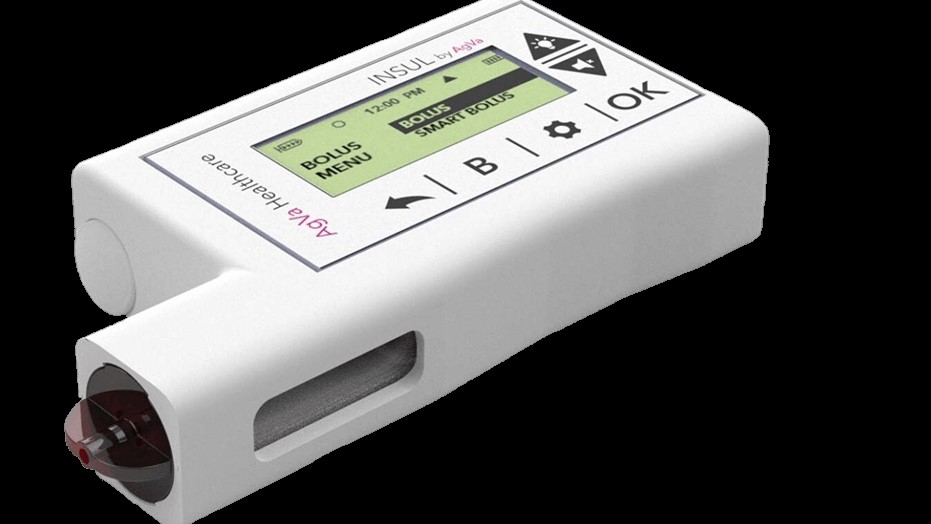
\includegraphics[width=\textwidth]{fig/lec14/Insulin_pump.jpg}
				\column{.2\linewidth}
				\caption*{Medication control (source: \href{https://commons.wikimedia.org/wiki/File:Insulin_pump.png}{www.wikipedia.org}, \href{https://creativecommons.org/licenses/by-sa/4.0/deed.en}{CC BY-SA 4.0})}
      \end{columns}
    \end{figure}
}

%%%%%%%%%%%%%%%%%%%%%%%%%%%%%%%%%%%%%%%%%%%%%%%%%%%%%%%%%%%%%
%% Safety levels %%
%%%%%%%%%%%%%%%%%%%%%%%%%%%%%%%%%%%%%%%%%%%%%%%%%%%%%%%%%%%%%
\frame{\frametitle{Safety levels}
\begin{figure}
\centering
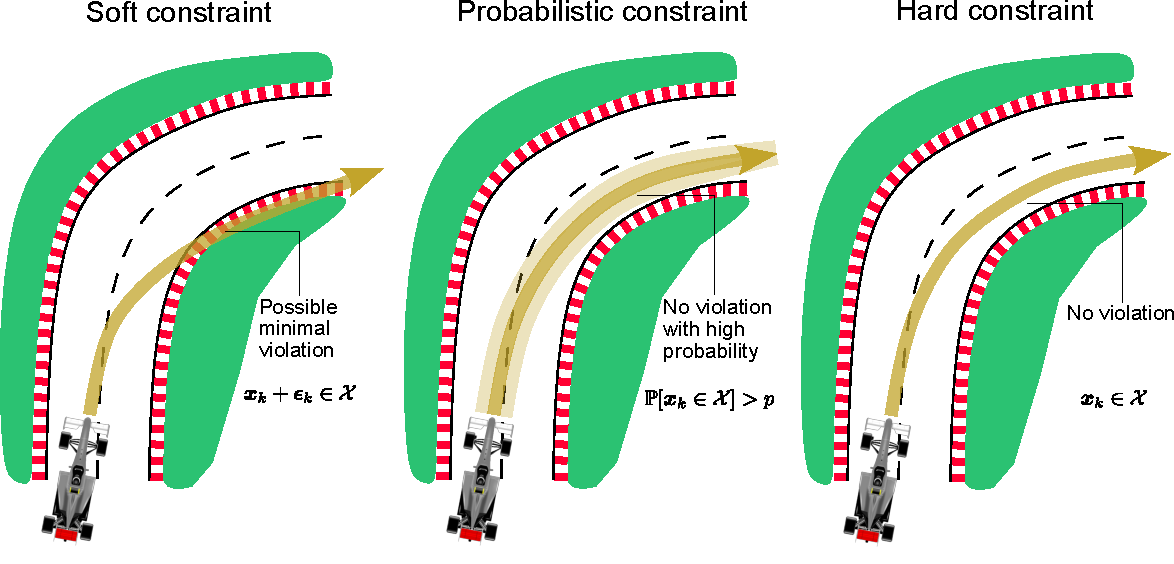
\includegraphics[height=0.68\textheight]{fig/lec14/Safety_Levels.pdf}
\caption{Different levels of safety (derived from L. Brunke et al., \textit{Safe Learning in Robotics: From Learning-Based Control to Safe Reinforcement Learning}, Annual Review of Control, Robotics, and Autonomous Systems, 2022)}
\label{fig:safety_levels}
\end{figure}
}

%%%%%%%%%%%%%%%%%%%%%%%%%%%%%%%%%%%%%%%%%%%%%%%%%%%%%%%%%%%%%
%% Bird's eye view on RL concepts integrating safety %%
%%%%%%%%%%%%%%%%%%%%%%%%%%%%%%%%%%%%%%%%%%%%%%%%%%%%%%%%%%%%%
\frame{\frametitle{Bird's eye view on RL concepts integrating safety}
\vspace{-0.1cm}
\begin{figure}%
\centering
\subfloat[][Safety critic: add a critic which indicates to which extent the current data sample fits to a safe situation]{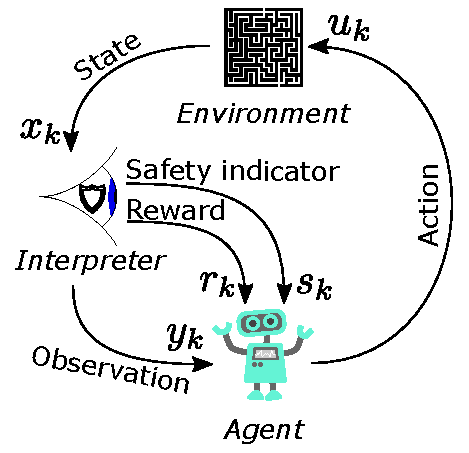
\includegraphics[width=0.375\textwidth]{fig/lec14/RL_Safety_Critic.pdf}}%
\qquad
\subfloat[][Safety shield: use a priori or learned model knowledge of the environment to make predictions identifying actions leading to unsafe situations]{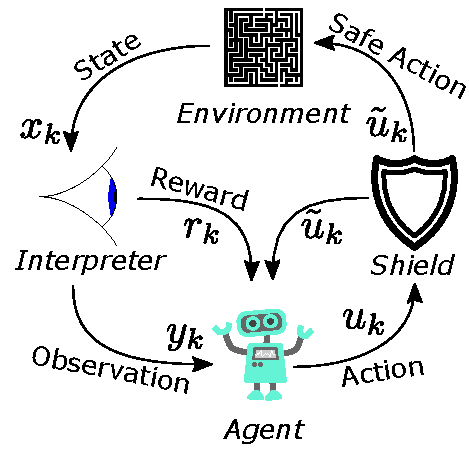
\includegraphics[width=0.375\textwidth]{fig/lec14/Safe_RL_Shield.pdf}}%
\label{fig:safety_birds_eye}%
\end{figure}
}

%%%%%%%%%%%%%%%%%%%%%%%%%%%%%%%%%%%%%%%%%%%%%%%%%%%%%%%%%%%%%
%% Bird's eye view on RL concepts integrating safety %%
%%%%%%%%%%%%%%%%%%%%%%%%%%%%%%%%%%%%%%%%%%%%%%%%%%%%%%%%%%%%%
\frame{\frametitle{Achievable safety levels and model knowledge}
\begin{figure}
\centering
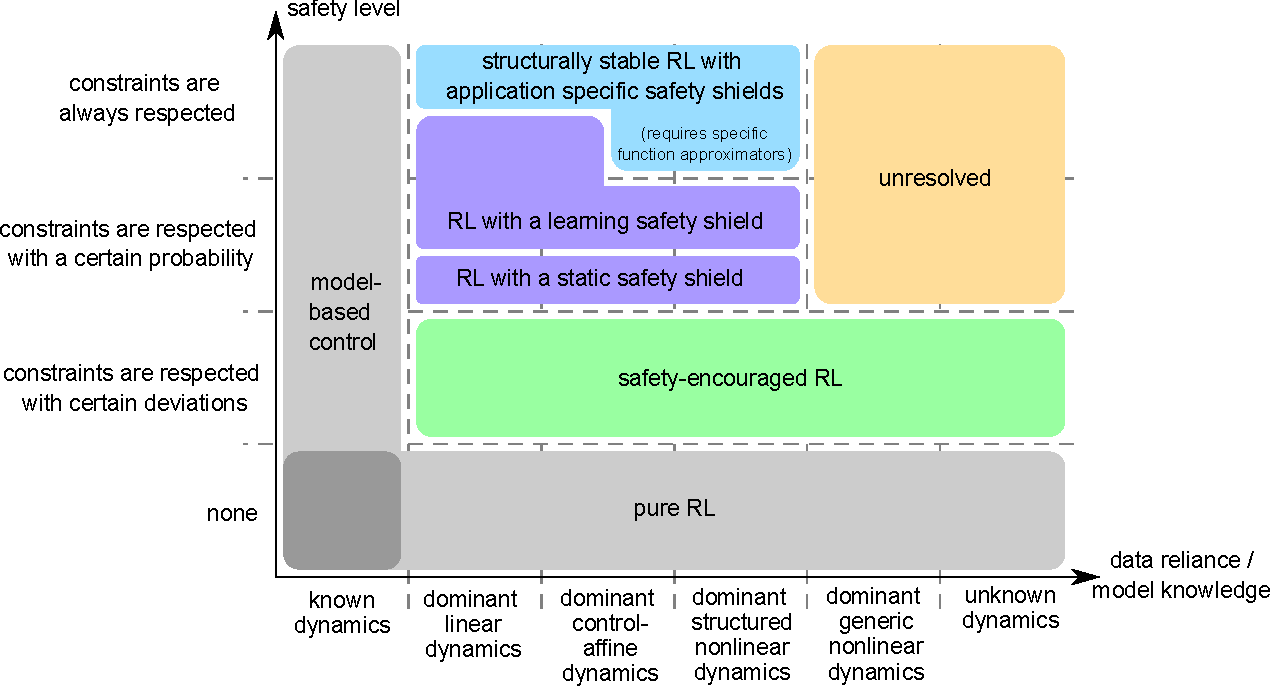
\includegraphics[height=0.68\textheight]{fig/lec14/Safeguard_Classes.pdf}
\caption{Safety and model knowledge map (derived from L. Brunke et al., \textit{Safe Learning in Robotics: From Learning-Based Control to Safe Reinforcement Learning}, Annual Review of Control, Robotics, and Autonomous Systems, 2022)}
\label{fig:safety_levels}
\end{figure}
}

%%%%%%%%%%%%%%%%%%%%%%%%%%%%%%%%%%%%%%%%%%%%%%%%%%%%%%%%%%%%%
%% MG Safe application %%
%%%%%%%%%%%%%%%%%%%%%%%%%%%%%%%%%%%%%%%%%%%%%%%%%%%%%%%%%%%%%
\frame{\frametitle{Energy system control application}
\vspace{-0.1cm}
\begin{figure}%
\centering
\subfloat[][\href{https://ei.uni-paderborn.de/lea/research/forschungsprojekte/intelligent-energy-systems/microgrid-laboratory}{LEA Microgrid Laboratory} showing inverter unit and control room]{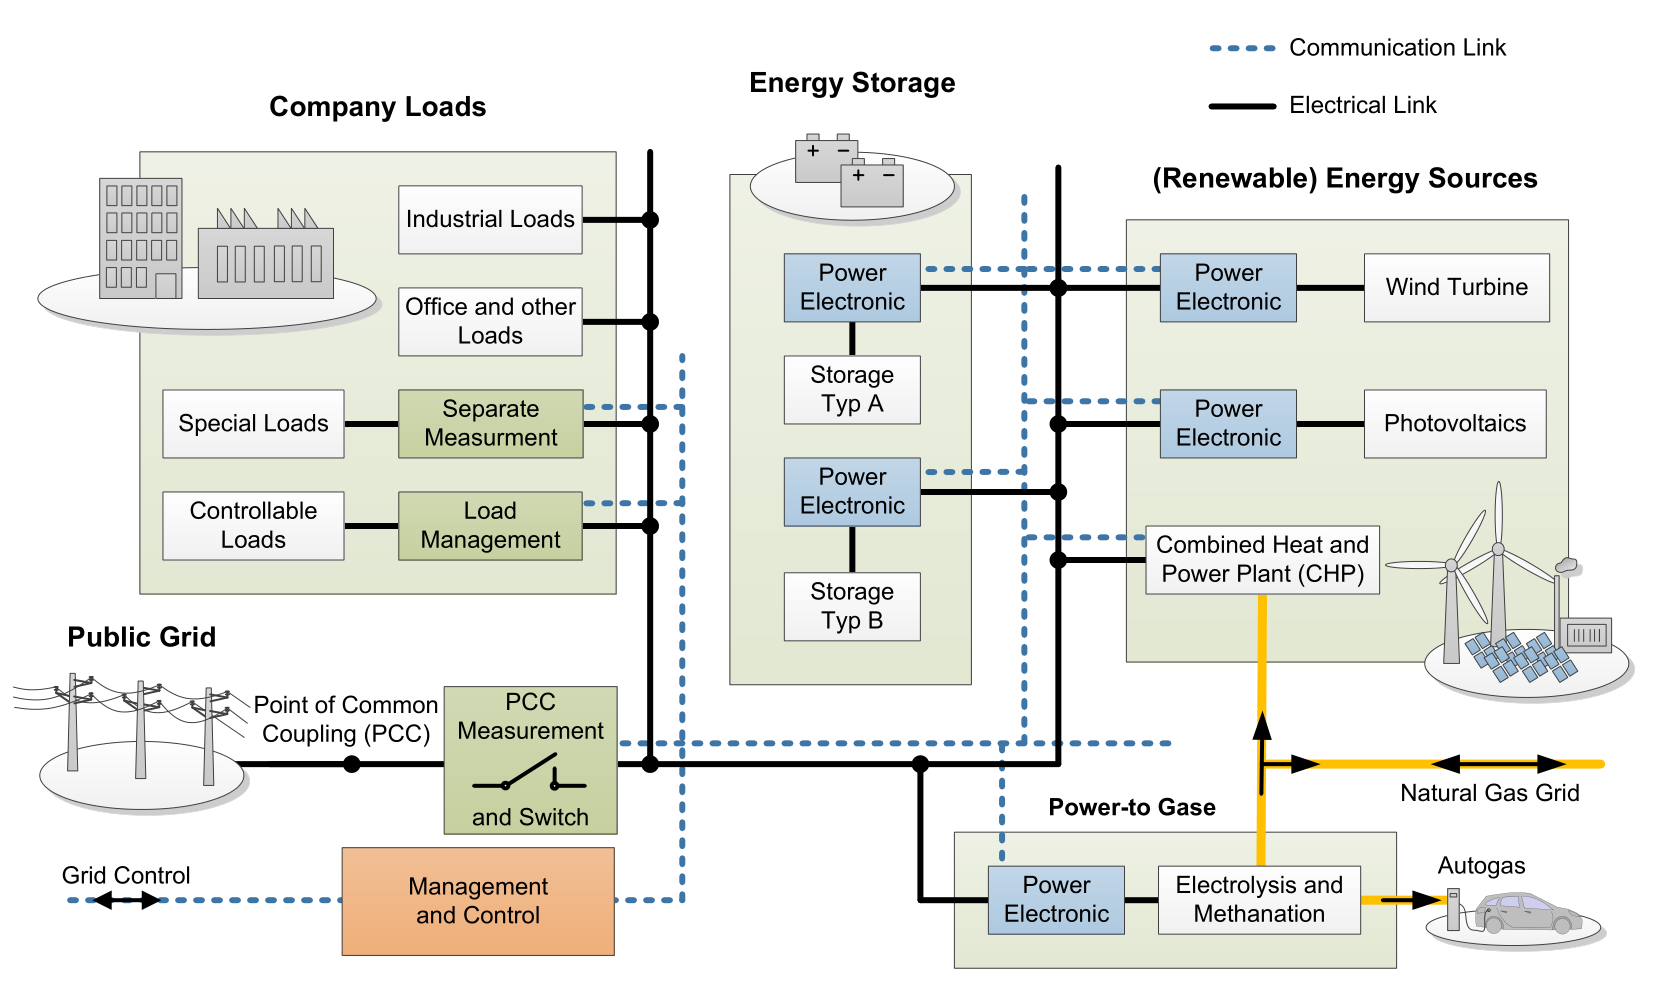
\includegraphics[width=0.45\textwidth]{fig/lec14/MG_vogt.png}}%
\qquad
\subfloat[][Application under investigation: Three-phase grid-forming inverter disturbed by stochastic load]{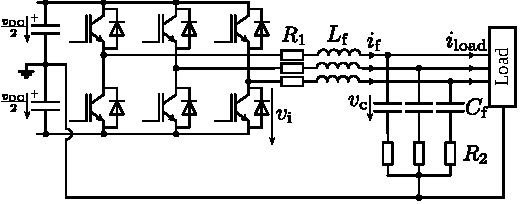
\includegraphics[width=0.45\textwidth]{fig/lec14/UPS_LC_Structure.pdf}}%
\label{fig:MG_application}%
\end{figure}
}


%%%%%%%%%%%%%%%%%%%%%%%%%%%%%%%%%%%%%%%%%%%%%%%%%%%%%%%%%%%%%
%% OMG + system constraints%%
%%%%%%%%%%%%%%%%%%%%%%%%%%%%%%%%%%%%%%%%%%%%%%%%%%%%%%%%%%%%%
\frame{\frametitle{Reference tracking with disturbance rejection}
\begin{columns}[t,onlytextwidth]
\begin{column}{0.475\textwidth}
\begin{minipage}[c]{\linewidth}
\begin{figure}
	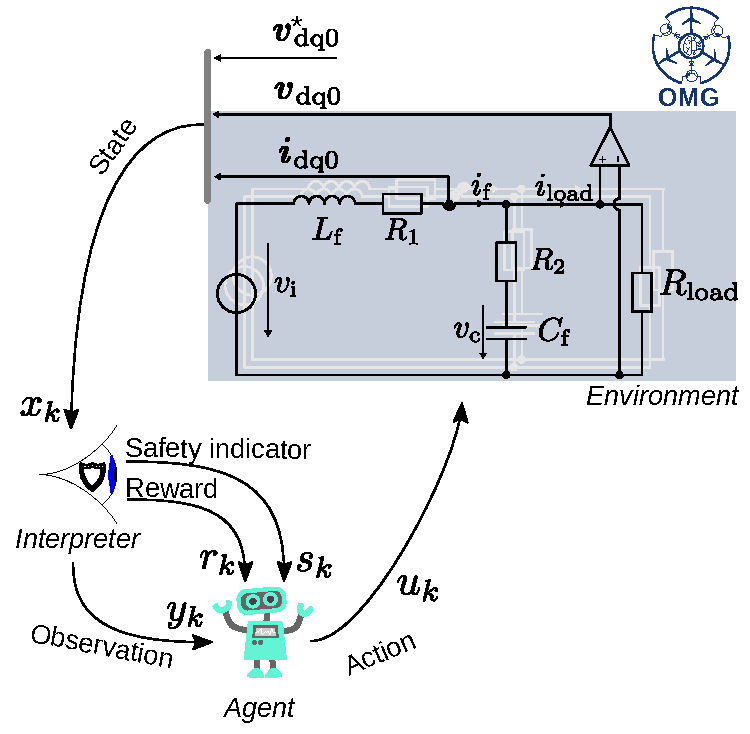
\includegraphics[width=0.8\textwidth, height=0.65\textheight]{fig/lec14/RL_Safety_Critic_OMG.pdf}
	\caption{Simulation setting with environment modeled using \href{https://github.com/upb-lea/openmodelica-microgrid-gym}{OpenModelica Microgrid Gym}}
	\label{fig:RL_OMG}
\end{figure}
\end{minipage}
\end{column}
\hfill
\begin{column}{0.54\textwidth}
\begin{minipage}[c]{\linewidth}
\begin{itemize}
	\item Cont. state- and actionspace
	\item Deep deterministic policy gradient agent
	\item Gird-forming inverter
	\item Stochastic load acts as disturbance
	\item State per phase: $\bm{x_k} = [i_\mathrm{f}, v_\mathrm{C_\mathrm{}}]$, $v_\mathrm{i} = v_\mathrm{DC} \cdot u_{k\mathrm{}}$
	\item $r_k=f(v_\mathrm{C}, v^*, i_\mathrm{f}) \in [1, -0.75]$
	%, i.e., goal is to supply load with voltage $v^*$
	\item $s_k = -1$, if limit ($i_\mathrm{f} \text{ or } v_\mathrm{C_\mathrm{}}$) is exceeded
\end{itemize}
\end{minipage}
\end{column}
\end{columns}
}

%%%%%%%%%%%%%%%%%%%%%%%%%%%%%%%%%%%%%%%%%%%%%%%%%%%%%%%%%%%%%
%% Reward function grid application
%%%%%%%%%%%%%%%%%%%%%%%%%%%%%%%%%%%%%%%%%%%%%%%%%%%%%%%%%%%%%
\frame{\frametitle{Reward design for grid-forming inverter}
\begin{columns}[t,onlytextwidth]
\begin{column}{0.475\textwidth}
\begin{minipage}[c]{\linewidth}
\begin{figure}
	%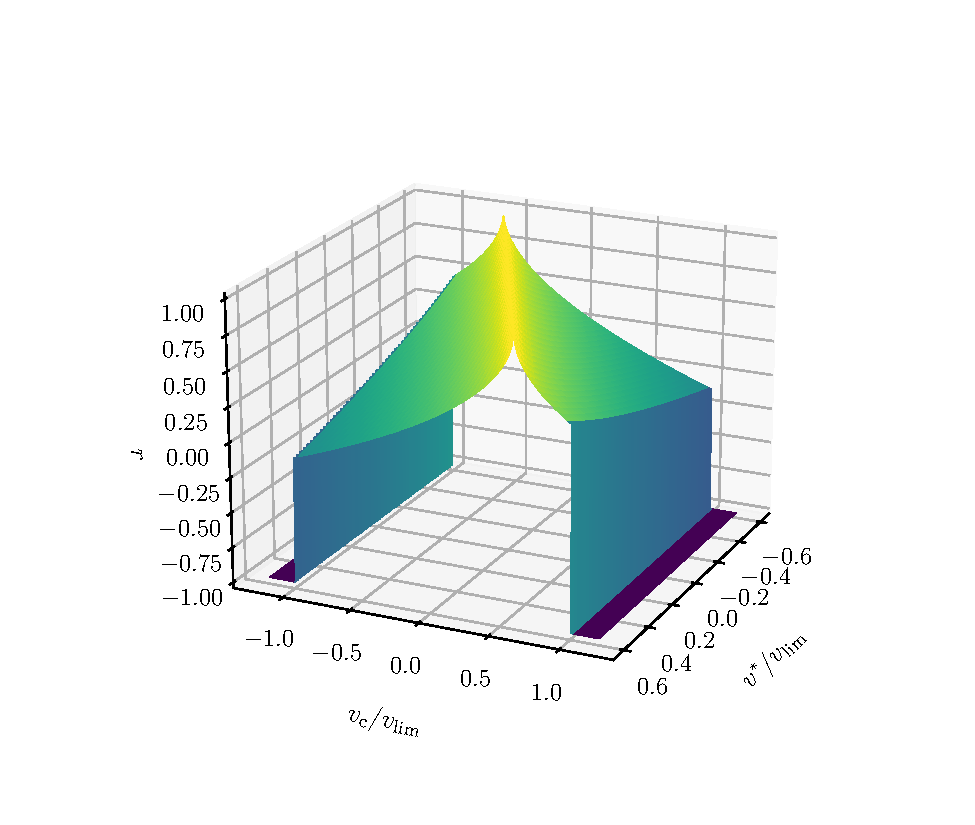
\includegraphics[width=1.11\textwidth, height=0.8\textheight]{fig/lec14/Reward_v_mre.pdf}
	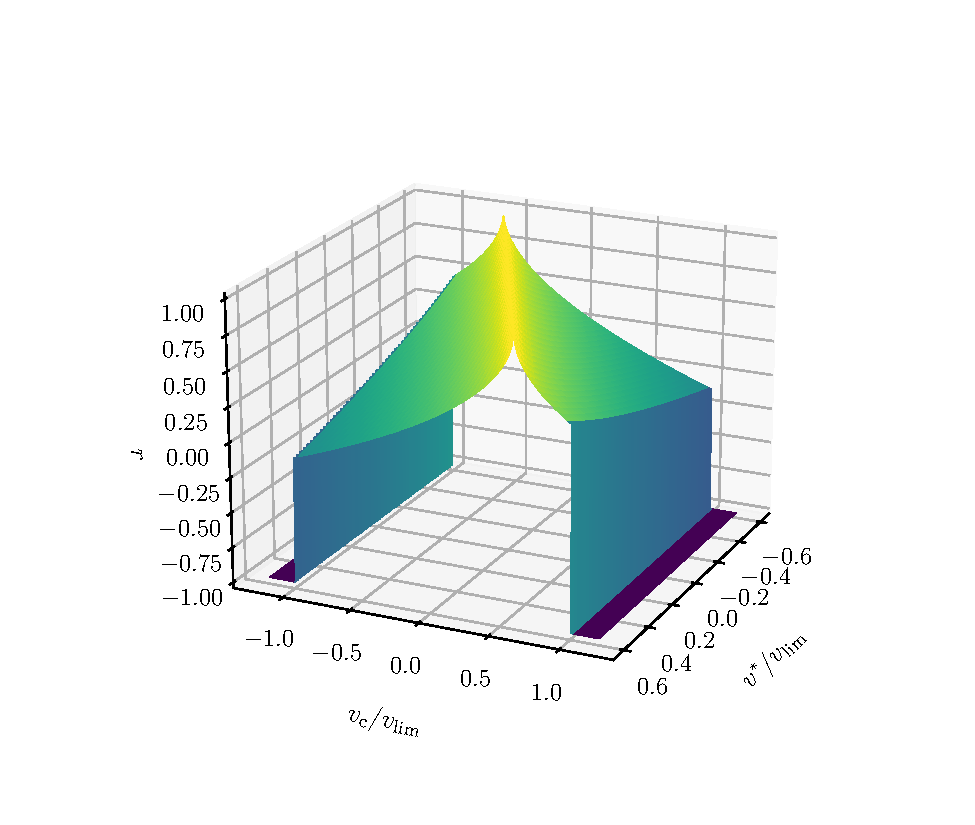
\includegraphics[trim=50 40 10 60, clip, width=1.1\linewidth]{fig/lec14/Reward_v_mre.pdf}
	\caption{Reward function \ref{eq:reward} for different reference and measured voltages and currents below nominal current \begin{tikzpicture}[auto,node distance=1cm,thin]
			%\tikzstyle{every node}=[shape=circle,fill=blue!10,draw=none, text=white,shading=ball]
			\tikzstyle{every node}=[shape=star,star point height=.2cm,fill=blue!50,draw=none, text=white,shading=ball]
			\node (1) {1};
		\end{tikzpicture} \& \begin{tikzpicture}[auto,node distance=1cm,thin]
			%\tikzstyle{every node}=[shape=circle,fill=blue!10,draw=none, text=white,shading=ball]
			\tikzstyle{every node}=[shape=star,star point height=.4cm,fill=blue!50,draw=none, text=white,shading=ball]
			\node (3) {3};
		\end{tikzpicture}}
	\label{fig:RL_OMG}
\end{figure}
\end{minipage}
\end{column}
\hfill
\begin{column}{0.54\textwidth}
\begin{minipage}[c]{\linewidth}
\begin{itemize}
	\item Three cases, depending on operation point
\end{itemize}
\begin{align}
    r_{} =
    \begin{cases}
         \text{MRE}(v_\mathrm{C}, v^*) , &
         \begin{tikzpicture}[auto,node distance=1cm,thin]
			\tikzstyle{every node}=[shape=star,star point height=.4cm,fill=blue!50,draw=none, text=white,shading=ball]
			\node (1) {1};
		\end{tikzpicture} \\
         %
         \text{MRE}(v_\mathrm{C}, v^*) + f(i_\mathrm{f}), & \begin{tikzpicture}[auto,node distance=1cm,thin]
			%\tikzstyle{every node}=[shape=circle,fill=blue!10,draw=none, text=white,shading=ball]
			\tikzstyle{every node}=[shape=star,star point height=.4cm,fill=blue!50,draw=none, text=white,shading=ball]
			\node (2) {2};
		\end{tikzpicture} \\
         %
         -1, & \begin{tikzpicture}[auto,node distance=1cm,thin]
			%\tikzstyle{every node}=[shape=circle,fill=blue!10,draw=none, text=white,shading=ball]
			\tikzstyle{every node}=[shape=star,star point height=.4cm,fill=blue!50,draw=none, text=white,shading=ball]
			\node (3) {3};
		\end{tikzpicture}
    \end{cases}
    \label{eq:reward}
\end{align}
\begin{itemize}
	\item \begin{tikzpicture}[auto,node distance=1cm,thin]
			\tikzstyle{every node}=[shape=star,star point height=.4cm,fill=blue!50,draw=none, text=white,shading=ball]
			\node (1) {1};
		\end{tikzpicture} $v_{\text{C}} \leq v_\mathrm{lim} \, \wedge\,  i_{\text{f}} \leq i_\mathrm{nom}$
	\item \begin{tikzpicture}[auto,node distance=1cm,thin]
			\tikzstyle{every node}=[shape=star,star point height=.4cm,fill=blue!50,draw=none, text=white,shading=ball]
			\node (2) {2};
		\end{tikzpicture} $v_{\text{C}} \leq v_\mathrm{lim} \, \wedge\, i_\mathrm{nom} \leq i_{\text{f}} \leq i_\mathrm{lim}$
	\item \begin{tikzpicture}[auto,node distance=1cm,thin]
			\tikzstyle{every node}=[shape=star,star point height=.4cm,fill=blue!50,draw=none, text=white,shading=ball]
			\node (3) {3};
		\end{tikzpicture} otherwise
	\item Linear punishment term $f(i_\mathrm{f})$
\end{itemize}
\end{minipage}
\end{column}
\end{columns}
}

%%%%%%%%%%%%%%%%%%%%%%%%%%%%%%%%%%%%%%%%%%%%%%%%%%%%%%%%%%%%%
%% OMG + safeguard%%
%%%%%%%%%%%%%%%%%%%%%%%%%%%%%%%%%%%%%%%%%%%%%%%%%%%%%%%%%%%%%
\frame{\frametitle{Reference tracking with disturbance rejection using saftey shield}
\begin{columns}[t,onlytextwidth]
\begin{column}{0.475\textwidth}
\begin{minipage}[c]{\linewidth}
\begin{figure}
	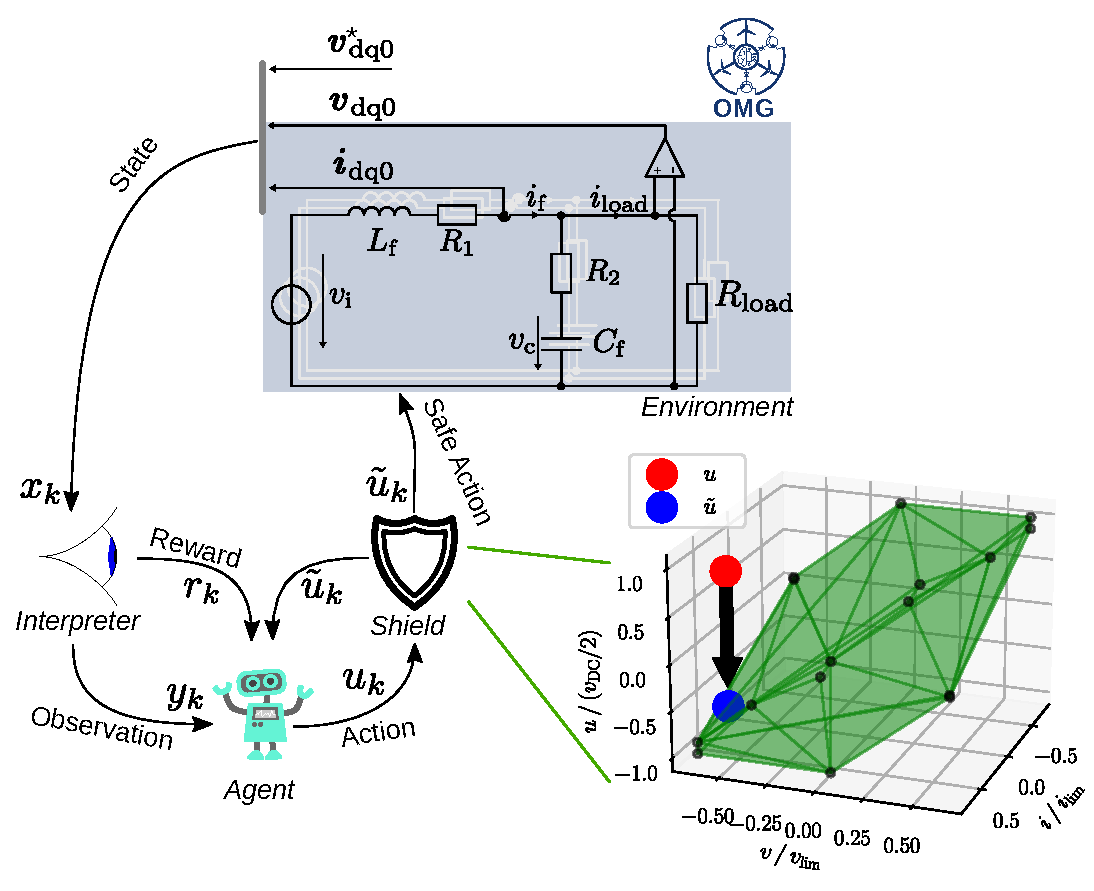
\includegraphics[width=0.9\textwidth, height=0.65\textheight]{fig/lec14/Safe_RL_Shield_OMG.pdf}
	\caption{Safety shield based on feasible set}
	\label{fig:RL_OMG}
\end{figure}
\end{minipage}
\end{column}
\hfill
\begin{column}{0.54\textwidth}
\begin{minipage}[c]{\linewidth}
\begin{itemize}
	\item Safety shield: Ensure that action does not cause state limit violation in future system trajectories
	\item Such a state action pair is called feasible
	\item Calculation of \textcolor{mygreen}{feasible set} requires a model
	\item Training data can be utilized to \href{https://ei.uni-paderborn.de/en/lea/teaching/veranstaltungen/teaching/translate-to-english-systemidentifikation}{identify} model
	\item Here, recursive least squares (RLS) is applied
\end{itemize}
\end{minipage}
\end{column}
\end{columns}
}

%%%%%%%%%%%%%%%%%%%%%%%%%%%%%%%%%%%%%%%%%%%%%%%%%%%%%%%%%%%%%
%% OMG + safeguard results%%
%%%%%%%%%%%%%%%%%%%%%%%%%%%%%%%%%%%%%%%%%%%%%%%%%%%%%%%%%%%%%
\frame{\frametitle{Saftey shield based on feasible set - proof of concept (1)}
\begin{columns}[t,onlytextwidth]
\begin{column}{0.475\textwidth}
\begin{minipage}[c]{\linewidth}
\begin{figure}
	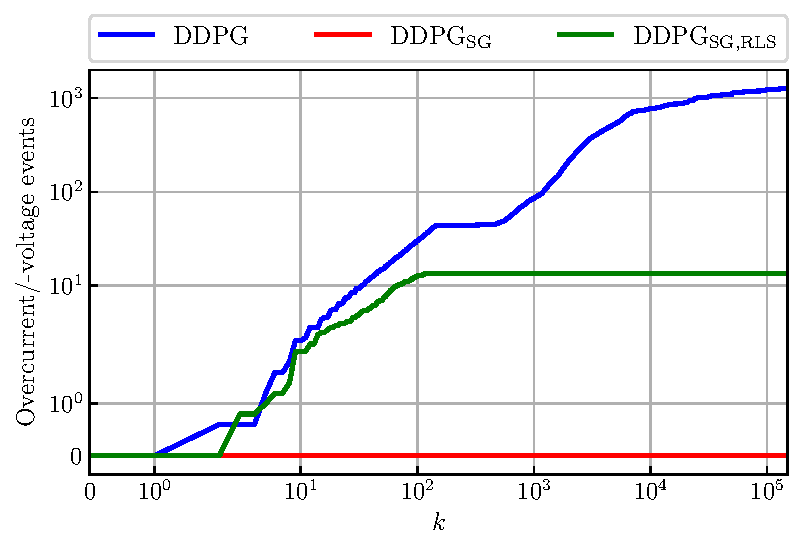
\includegraphics[width=0.85\textwidth, height=0.55\textheight]{fig/lec14/OMG_all_aborts_log.pdf}
	\caption{Accumulated unsafe events (overcurrent/-voltage) per trainingstep $k$}
	\label{fig:RL_OMG}
\end{figure}
\end{minipage}
\end{column}
\hfill
\begin{column}{0.54\textwidth}
\begin{minipage}[c]{\linewidth}
\begin{itemize}
	\item Three different approaches
	\item \textcolor{blue}{$\mathrm{DDPG}_\mathrm{}$}: Agent without safety shield
	\item \textcolor{red}{$\mathrm{DDPG}_\mathrm{SG}$}: Agent with safety shield using perfect a priori knowledge
	\item \textcolor{mygreen}{$\mathrm{DDPG}_\mathrm{SG,RLS}$}: Agent with safety shield without a priori knowledge, identifying model using RLS
	\item Five agents trained per approach
	\item Results in D. Weber et al., \textit{Safe Reinforcement Learning-Based Control in
Power Electronic Systems}, 2023
\end{itemize}
\end{minipage}
\end{column}
\end{columns}
}

%%%%%%%%%%%%%%%%%%%%%%%%%%%%%%%%%%%%%%%%%%%%%%%%%%%%%%%%%%%%%
%% OMG + safeguard results%%
%%%%%%%%%%%%%%%%%%%%%%%%%%%%%%%%%%%%%%%%%%%%%%%%%%%%%%%%%%%%%
\frame{\frametitle{Saftey shield based on feasible set - proof of concept (2)}
\begin{columns}[t,onlytextwidth]
\begin{column}{0.54\textwidth}
\begin{minipage}[c]{\linewidth}
\begin{figure}
	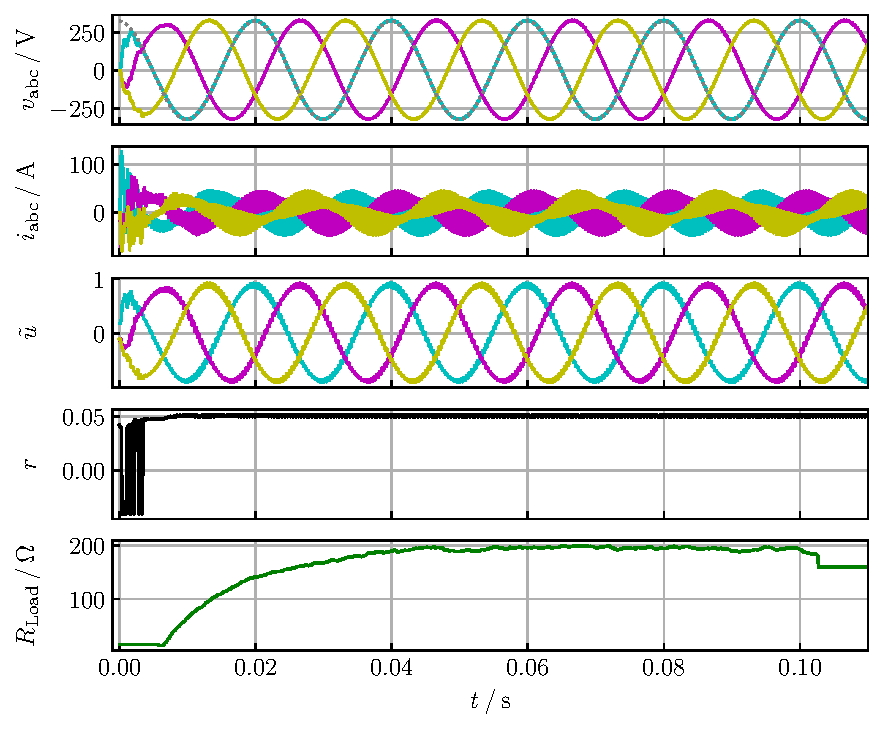
\includegraphics[width=0.75\textwidth, height=0.55\textheight]{fig/lec14/370_vDC_SL_RLS_varLoadtimeseries_testcase.pdf}
	\caption{Blackstart after training using \textcolor{mygreen}{$\mathrm{DDPG}_\mathrm{SG,RLS}$}}
	\label{fig:RL_OMG}
\end{figure}
\end{minipage}
\end{column}
\hfill
\begin{column}{0.45\textwidth}
\begin{minipage}[c]{\linewidth}
\begin{itemize}
	\item $\mathrm{DDPG}_\mathrm{SG,RLS}$ agent trained for 150000 steps
	\item $R_\mathrm{Load}$ changes every step based on random process
	\item Additional events -- load steps and drifts -- trigged randomly
\end{itemize}
\end{minipage}
\end{column}
\end{columns}
}

%%%%%%%%%%%%%%%%%%%%%%%%%%%%%%%%%%%%%%%%%%%%%%%%%%%%%%%%%%%%%%%%%%
\section{Real-World Implementation with Fast Policy Inference} 
%%%%%%%%%%%%%%%%%%%%%%%%%%%%%%%%%%%%%%%%%%%%%%%%%%%%%%%%%%%%%%%%%%
\begin{frame}
\frametitle{Table of contents}
\tableofcontents[currentsection]
\end{frame}

%%%%%%%%%%%%%%%%%%%%%%%%%%%%%%%%%%%%%%%%%%%%%%%%%%%%%%%%%%%%%
%% Real-time implementation aspects %%
%%%%%%%%%%%%%%%%%%%%%%%%%%%%%%%%%%%%%%%%%%%%%%%%%%%%%%%%%%%%%
\frame{\frametitle{Real-time implementation aspects (1)}
\begin{figure}
\centering
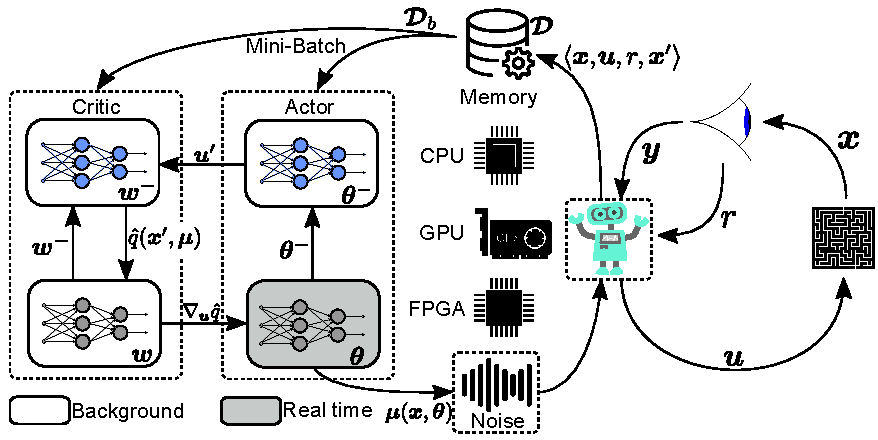
\includegraphics[height=0.68\textheight]{fig/lec14/DDPG_Real_Time.pdf}
\caption{DDPG implementation example (derivative work of \figref{fig:RL_Wiki} and \href{https://commons.wikimedia.org/wiki/File:Multi-Layer_Neural_Network-Vector.svg?uselang=de}{wikipedia.org}, \href{https://creativecommons.org/publicdomain/zero/1.0/deed.en}{CC0 1.0})}
\label{fig:DDPG_Real_Time}
\end{figure}
}

%%%%%%%%%%%%%%%%%%%%%%%%%%%%%%%%%%%%%%%%%%%%%%%%%%%%%%%%%%%%%
%% Bird's eye view on RL concepts integrating safety %%
%%%%%%%%%%%%%%%%%%%%%%%%%%%%%%%%%%%%%%%%%%%%%%%%%%%%%%%%%%%%%
\frame{\frametitle{Real-time implementation aspects (2)}
\vspace{-0.1cm}
\begin{figure}%
\centering
\subfloat[][Real-time control requirement vs. learning time]{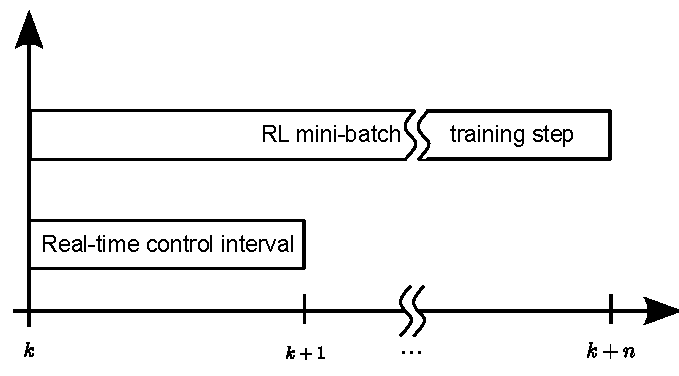
\includegraphics[width=0.45\textwidth]{fig/lec14/Timing.pdf}}%
\qquad
\subfloat[][Typical evolution of RL parameter weights during learning]{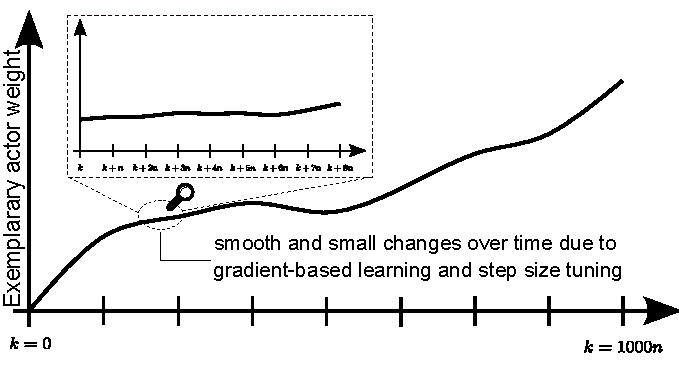
\includegraphics[width=0.45\textwidth]{fig/lec14/NN-Weights.pdf}}%
\label{fig:timing}%
\end{figure}
}

%%%%%%%%%%%%%%%%%%%%%%%%%%%%%%%%%%%%%%%%%%%%%%%%%%%%%%%%%%%%%%%%%%
\section{Meta Reinforcement Learning} 
%%%%%%%%%%%%%%%%%%%%%%%%%%%%%%%%%%%%%%%%%%%%%%%%%%%%%%%%%%%%%%%%%%
\begin{frame}
\frametitle{Table of contents}
\tableofcontents[currentsection]
\end{frame}
